
% Default to the notebook output style

    


% Inherit from the specified cell style.




\renewcommand{\familydefault}{\sfdefault}

\documentclass[11pt]{article}


    \usepackage{graphicx}
    \graphicspath{ {images/} }
    
    \usepackage{fancyhdr}
    
    \usepackage[T1]{fontenc}
    % Nicer default font than Computer Modern for most use cases
    \usepackage{palatino}

    % Basic figure setup, for now with no caption control since it's done
    % automatically by Pandoc (which extracts ![](path) syntax from Markdown).
    \usepackage{graphicx}
    % We will generate all images so they have a width \maxwidth. This means
    % that they will get their normal width if they fit onto the page, but
    % are scaled down if they would overflow the margins.
    \makeatletter
    \def\maxwidth{\ifdim\Gin@nat@width>\linewidth\linewidth
    \else\Gin@nat@width\fi}
    \makeatother
    %\let\Oldincludegraphics\includegraphics
    % Set max figure width to be 80% of text width, for now hardcoded.
    %\renewcommand{\includegraphics}[1]{\Oldincludegraphics[width=.8\maxwidth]{#1}}
    % Ensure that by default, figures have no caption (until we provide a
    % proper Figure object with a Caption API and a way to capture that
    % in the conversion process - todo).
    \usepackage{caption}
    \DeclareCaptionLabelFormat{nolabel}{}
    \captionsetup{labelformat=nolabel}

    \usepackage{adjustbox} % Used to constrain images to a maximum size 
    \usepackage{xcolor} % Allow colors to be defined
    \usepackage{enumerate} % Needed for markdown enumerations to work
    \usepackage{geometry} % Used to adjust the document margins
    \usepackage{amsmath} % Equations
    \usepackage{amssymb} % Equations
    \usepackage{textcomp} % defines textquotesingle
    % Hack from http://tex.stackexchange.com/a/47451/13684:
    \AtBeginDocument{%
        \def\PYZsq{\textquotesingle}% Upright quotes in Pygmentized code
    }
    \usepackage{upquote} % Upright quotes for verbatim code
    \usepackage{eurosym} % defines \euro
    \usepackage[mathletters]{ucs} % Extended unicode (utf-8) support
    \usepackage[utf8x]{inputenc} % Allow utf-8 characters in the tex document
    \usepackage{fancyvrb} % verbatim replacement that allows latex
    \usepackage{grffile} % extends the file name processing of package graphics 
                         % to support a larger range 
    % The hyperref package gives us a pdf with properly built
    % internal navigation ('pdf bookmarks' for the table of contents,
    % internal cross-reference links, web links for URLs, etc.)
    \usepackage{hyperref}
    \usepackage{longtable} % longtable support required by pandoc >1.10
    \usepackage{booktabs}  % table support for pandoc > 1.12.2
    \usepackage[normalem]{ulem} % ulem is needed to support strikethroughs (\sout)
                                % normalem makes italics be italics, not underlines
    

    
    
    % Colors for the hyperref package
    \definecolor{urlcolor}{rgb}{0,.145,.698}
    \definecolor{linkcolor}{rgb}{.71,0.21,0.01}
    \definecolor{citecolor}{rgb}{.12,.54,.11}

    % ANSI colors
    \definecolor{ansi-black}{HTML}{3E424D}
    \definecolor{ansi-black-intense}{HTML}{282C36}
    \definecolor{ansi-red}{HTML}{E75C58}
    \definecolor{ansi-red-intense}{HTML}{B22B31}
    \definecolor{ansi-green}{HTML}{00A250}
    \definecolor{ansi-green-intense}{HTML}{007427}
    \definecolor{ansi-yellow}{HTML}{DDB62B}
    \definecolor{ansi-yellow-intense}{HTML}{B27D12}
    \definecolor{ansi-blue}{HTML}{208FFB}
    \definecolor{ansi-blue-intense}{HTML}{0065CA}
    \definecolor{ansi-magenta}{HTML}{D160C4}
    \definecolor{ansi-magenta-intense}{HTML}{A03196}
    \definecolor{ansi-cyan}{HTML}{60C6C8}
    \definecolor{ansi-cyan-intense}{HTML}{258F8F}
    \definecolor{ansi-white}{HTML}{C5C1B4}
    \definecolor{ansi-white-intense}{HTML}{A1A6B2}

    % commands and environments needed by pandoc snippets
    % extracted from the output of `pandoc -s`
    \providecommand{\tightlist}{%
      \setlength{\itemsep}{0pt}\setlength{\parskip}{0pt}}
    \DefineVerbatimEnvironment{Highlighting}{Verbatim}{commandchars=\\\{\}}
    % Add ',fontsize=\small' for more characters per line
    \newenvironment{Shaded}{}{}
    \newcommand{\KeywordTok}[1]{\textcolor[rgb]{0.00,0.44,0.13}{\textbf{{#1}}}}
    \newcommand{\DataTypeTok}[1]{\textcolor[rgb]{0.56,0.13,0.00}{{#1}}}
    \newcommand{\DecValTok}[1]{\textcolor[rgb]{0.25,0.63,0.44}{{#1}}}
    \newcommand{\BaseNTok}[1]{\textcolor[rgb]{0.25,0.63,0.44}{{#1}}}
    \newcommand{\FloatTok}[1]{\textcolor[rgb]{0.25,0.63,0.44}{{#1}}}
    \newcommand{\CharTok}[1]{\textcolor[rgb]{0.25,0.44,0.63}{{#1}}}
    \newcommand{\StringTok}[1]{\textcolor[rgb]{0.25,0.44,0.63}{{#1}}}
    \newcommand{\CommentTok}[1]{\textcolor[rgb]{0.38,0.63,0.69}{\textit{{#1}}}}
    \newcommand{\OtherTok}[1]{\textcolor[rgb]{0.00,0.44,0.13}{{#1}}}
    \newcommand{\AlertTok}[1]{\textcolor[rgb]{1.00,0.00,0.00}{\textbf{{#1}}}}
    \newcommand{\FunctionTok}[1]{\textcolor[rgb]{0.02,0.16,0.49}{{#1}}}
    \newcommand{\RegionMarkerTok}[1]{{#1}}
    \newcommand{\ErrorTok}[1]{\textcolor[rgb]{1.00,0.00,0.00}{\textbf{{#1}}}}
    \newcommand{\NormalTok}[1]{{#1}}
    
    % Additional commands for more recent versions of Pandoc
    \newcommand{\ConstantTok}[1]{\textcolor[rgb]{0.53,0.00,0.00}{{#1}}}
    \newcommand{\SpecialCharTok}[1]{\textcolor[rgb]{0.25,0.44,0.63}{{#1}}}
    \newcommand{\VerbatimStringTok}[1]{\textcolor[rgb]{0.25,0.44,0.63}{{#1}}}
    \newcommand{\SpecialStringTok}[1]{\textcolor[rgb]{0.73,0.40,0.53}{{#1}}}
    \newcommand{\ImportTok}[1]{{#1}}
    \newcommand{\DocumentationTok}[1]{\textcolor[rgb]{0.73,0.13,0.13}{\textit{{#1}}}}
    \newcommand{\AnnotationTok}[1]{\textcolor[rgb]{0.38,0.63,0.69}{\textbf{\textit{{#1}}}}}
    \newcommand{\CommentVarTok}[1]{\textcolor[rgb]{0.38,0.63,0.69}{\textbf{\textit{{#1}}}}}
    \newcommand{\VariableTok}[1]{\textcolor[rgb]{0.10,0.09,0.49}{{#1}}}
    \newcommand{\ControlFlowTok}[1]{\textcolor[rgb]{0.00,0.44,0.13}{\textbf{{#1}}}}
    \newcommand{\OperatorTok}[1]{\textcolor[rgb]{0.40,0.40,0.40}{{#1}}}
    \newcommand{\BuiltInTok}[1]{{#1}}
    \newcommand{\ExtensionTok}[1]{{#1}}
    \newcommand{\PreprocessorTok}[1]{\textcolor[rgb]{0.74,0.48,0.00}{{#1}}}
    \newcommand{\AttributeTok}[1]{\textcolor[rgb]{0.49,0.56,0.16}{{#1}}}
    \newcommand{\InformationTok}[1]{\textcolor[rgb]{0.38,0.63,0.69}{\textbf{\textit{{#1}}}}}
    \newcommand{\WarningTok}[1]{\textcolor[rgb]{0.38,0.63,0.69}{\textbf{\textit{{#1}}}}}
    
    
    % Define a nice break command that doesn't care if a line doesn't already
    % exist.
    \def\br{\hspace*{\fill} \\* }
    % Math Jax compatability definitions
    \def\gt{>}
    \def\lt{<}
    % Document parameters
    \title{Wrangling Singapore’s Geographic Data}
    
    
    

    % Pygments definitions
    
\makeatletter
\def\PY@reset{\let\PY@it=\relax \let\PY@bf=\relax%
    \let\PY@ul=\relax \let\PY@tc=\relax%
    \let\PY@bc=\relax \let\PY@ff=\relax}
\def\PY@tok#1{\csname PY@tok@#1\endcsname}
\def\PY@toks#1+{\ifx\relax#1\empty\else%
    \PY@tok{#1}\expandafter\PY@toks\fi}
\def\PY@do#1{\PY@bc{\PY@tc{\PY@ul{%
    \PY@it{\PY@bf{\PY@ff{#1}}}}}}}
\def\PY#1#2{\PY@reset\PY@toks#1+\relax+\PY@do{#2}}

\expandafter\def\csname PY@tok@gd\endcsname{\def\PY@tc##1{\textcolor[rgb]{0.63,0.00,0.00}{##1}}}
\expandafter\def\csname PY@tok@gu\endcsname{\let\PY@bf=\textbf\def\PY@tc##1{\textcolor[rgb]{0.50,0.00,0.50}{##1}}}
\expandafter\def\csname PY@tok@gt\endcsname{\def\PY@tc##1{\textcolor[rgb]{0.00,0.27,0.87}{##1}}}
\expandafter\def\csname PY@tok@gs\endcsname{\let\PY@bf=\textbf}
\expandafter\def\csname PY@tok@gr\endcsname{\def\PY@tc##1{\textcolor[rgb]{1.00,0.00,0.00}{##1}}}
\expandafter\def\csname PY@tok@cm\endcsname{\let\PY@it=\textit\def\PY@tc##1{\textcolor[rgb]{0.25,0.50,0.50}{##1}}}
\expandafter\def\csname PY@tok@vg\endcsname{\def\PY@tc##1{\textcolor[rgb]{0.10,0.09,0.49}{##1}}}
\expandafter\def\csname PY@tok@vi\endcsname{\def\PY@tc##1{\textcolor[rgb]{0.10,0.09,0.49}{##1}}}
\expandafter\def\csname PY@tok@mh\endcsname{\def\PY@tc##1{\textcolor[rgb]{0.40,0.40,0.40}{##1}}}
\expandafter\def\csname PY@tok@cs\endcsname{\let\PY@it=\textit\def\PY@tc##1{\textcolor[rgb]{0.25,0.50,0.50}{##1}}}
\expandafter\def\csname PY@tok@ge\endcsname{\let\PY@it=\textit}
\expandafter\def\csname PY@tok@vc\endcsname{\def\PY@tc##1{\textcolor[rgb]{0.10,0.09,0.49}{##1}}}
\expandafter\def\csname PY@tok@il\endcsname{\def\PY@tc##1{\textcolor[rgb]{0.40,0.40,0.40}{##1}}}
\expandafter\def\csname PY@tok@go\endcsname{\def\PY@tc##1{\textcolor[rgb]{0.53,0.53,0.53}{##1}}}
\expandafter\def\csname PY@tok@cp\endcsname{\def\PY@tc##1{\textcolor[rgb]{0.74,0.48,0.00}{##1}}}
\expandafter\def\csname PY@tok@gi\endcsname{\def\PY@tc##1{\textcolor[rgb]{0.00,0.63,0.00}{##1}}}
\expandafter\def\csname PY@tok@gh\endcsname{\let\PY@bf=\textbf\def\PY@tc##1{\textcolor[rgb]{0.00,0.00,0.50}{##1}}}
\expandafter\def\csname PY@tok@ni\endcsname{\let\PY@bf=\textbf\def\PY@tc##1{\textcolor[rgb]{0.60,0.60,0.60}{##1}}}
\expandafter\def\csname PY@tok@nl\endcsname{\def\PY@tc##1{\textcolor[rgb]{0.63,0.63,0.00}{##1}}}
\expandafter\def\csname PY@tok@nn\endcsname{\let\PY@bf=\textbf\def\PY@tc##1{\textcolor[rgb]{0.00,0.00,1.00}{##1}}}
\expandafter\def\csname PY@tok@no\endcsname{\def\PY@tc##1{\textcolor[rgb]{0.53,0.00,0.00}{##1}}}
\expandafter\def\csname PY@tok@na\endcsname{\def\PY@tc##1{\textcolor[rgb]{0.49,0.56,0.16}{##1}}}
\expandafter\def\csname PY@tok@nb\endcsname{\def\PY@tc##1{\textcolor[rgb]{0.00,0.50,0.00}{##1}}}
\expandafter\def\csname PY@tok@nc\endcsname{\let\PY@bf=\textbf\def\PY@tc##1{\textcolor[rgb]{0.00,0.00,1.00}{##1}}}
\expandafter\def\csname PY@tok@nd\endcsname{\def\PY@tc##1{\textcolor[rgb]{0.67,0.13,1.00}{##1}}}
\expandafter\def\csname PY@tok@ne\endcsname{\let\PY@bf=\textbf\def\PY@tc##1{\textcolor[rgb]{0.82,0.25,0.23}{##1}}}
\expandafter\def\csname PY@tok@nf\endcsname{\def\PY@tc##1{\textcolor[rgb]{0.00,0.00,1.00}{##1}}}
\expandafter\def\csname PY@tok@si\endcsname{\let\PY@bf=\textbf\def\PY@tc##1{\textcolor[rgb]{0.73,0.40,0.53}{##1}}}
\expandafter\def\csname PY@tok@s2\endcsname{\def\PY@tc##1{\textcolor[rgb]{0.73,0.13,0.13}{##1}}}
\expandafter\def\csname PY@tok@nt\endcsname{\let\PY@bf=\textbf\def\PY@tc##1{\textcolor[rgb]{0.00,0.50,0.00}{##1}}}
\expandafter\def\csname PY@tok@nv\endcsname{\def\PY@tc##1{\textcolor[rgb]{0.10,0.09,0.49}{##1}}}
\expandafter\def\csname PY@tok@s1\endcsname{\def\PY@tc##1{\textcolor[rgb]{0.73,0.13,0.13}{##1}}}
\expandafter\def\csname PY@tok@ch\endcsname{\let\PY@it=\textit\def\PY@tc##1{\textcolor[rgb]{0.25,0.50,0.50}{##1}}}
\expandafter\def\csname PY@tok@m\endcsname{\def\PY@tc##1{\textcolor[rgb]{0.40,0.40,0.40}{##1}}}
\expandafter\def\csname PY@tok@gp\endcsname{\let\PY@bf=\textbf\def\PY@tc##1{\textcolor[rgb]{0.00,0.00,0.50}{##1}}}
\expandafter\def\csname PY@tok@sh\endcsname{\def\PY@tc##1{\textcolor[rgb]{0.73,0.13,0.13}{##1}}}
\expandafter\def\csname PY@tok@ow\endcsname{\let\PY@bf=\textbf\def\PY@tc##1{\textcolor[rgb]{0.67,0.13,1.00}{##1}}}
\expandafter\def\csname PY@tok@sx\endcsname{\def\PY@tc##1{\textcolor[rgb]{0.00,0.50,0.00}{##1}}}
\expandafter\def\csname PY@tok@bp\endcsname{\def\PY@tc##1{\textcolor[rgb]{0.00,0.50,0.00}{##1}}}
\expandafter\def\csname PY@tok@c1\endcsname{\let\PY@it=\textit\def\PY@tc##1{\textcolor[rgb]{0.25,0.50,0.50}{##1}}}
\expandafter\def\csname PY@tok@o\endcsname{\def\PY@tc##1{\textcolor[rgb]{0.40,0.40,0.40}{##1}}}
\expandafter\def\csname PY@tok@kc\endcsname{\let\PY@bf=\textbf\def\PY@tc##1{\textcolor[rgb]{0.00,0.50,0.00}{##1}}}
\expandafter\def\csname PY@tok@c\endcsname{\let\PY@it=\textit\def\PY@tc##1{\textcolor[rgb]{0.25,0.50,0.50}{##1}}}
\expandafter\def\csname PY@tok@mf\endcsname{\def\PY@tc##1{\textcolor[rgb]{0.40,0.40,0.40}{##1}}}
\expandafter\def\csname PY@tok@err\endcsname{\def\PY@bc##1{\setlength{\fboxsep}{0pt}\fcolorbox[rgb]{1.00,0.00,0.00}{1,1,1}{\strut ##1}}}
\expandafter\def\csname PY@tok@mb\endcsname{\def\PY@tc##1{\textcolor[rgb]{0.40,0.40,0.40}{##1}}}
\expandafter\def\csname PY@tok@ss\endcsname{\def\PY@tc##1{\textcolor[rgb]{0.10,0.09,0.49}{##1}}}
\expandafter\def\csname PY@tok@sr\endcsname{\def\PY@tc##1{\textcolor[rgb]{0.73,0.40,0.53}{##1}}}
\expandafter\def\csname PY@tok@mo\endcsname{\def\PY@tc##1{\textcolor[rgb]{0.40,0.40,0.40}{##1}}}
\expandafter\def\csname PY@tok@kd\endcsname{\let\PY@bf=\textbf\def\PY@tc##1{\textcolor[rgb]{0.00,0.50,0.00}{##1}}}
\expandafter\def\csname PY@tok@mi\endcsname{\def\PY@tc##1{\textcolor[rgb]{0.40,0.40,0.40}{##1}}}
\expandafter\def\csname PY@tok@kn\endcsname{\let\PY@bf=\textbf\def\PY@tc##1{\textcolor[rgb]{0.00,0.50,0.00}{##1}}}
\expandafter\def\csname PY@tok@cpf\endcsname{\let\PY@it=\textit\def\PY@tc##1{\textcolor[rgb]{0.25,0.50,0.50}{##1}}}
\expandafter\def\csname PY@tok@kr\endcsname{\let\PY@bf=\textbf\def\PY@tc##1{\textcolor[rgb]{0.00,0.50,0.00}{##1}}}
\expandafter\def\csname PY@tok@s\endcsname{\def\PY@tc##1{\textcolor[rgb]{0.73,0.13,0.13}{##1}}}
\expandafter\def\csname PY@tok@kp\endcsname{\def\PY@tc##1{\textcolor[rgb]{0.00,0.50,0.00}{##1}}}
\expandafter\def\csname PY@tok@w\endcsname{\def\PY@tc##1{\textcolor[rgb]{0.73,0.73,0.73}{##1}}}
\expandafter\def\csname PY@tok@kt\endcsname{\def\PY@tc##1{\textcolor[rgb]{0.69,0.00,0.25}{##1}}}
\expandafter\def\csname PY@tok@sc\endcsname{\def\PY@tc##1{\textcolor[rgb]{0.73,0.13,0.13}{##1}}}
\expandafter\def\csname PY@tok@sb\endcsname{\def\PY@tc##1{\textcolor[rgb]{0.73,0.13,0.13}{##1}}}
\expandafter\def\csname PY@tok@k\endcsname{\let\PY@bf=\textbf\def\PY@tc##1{\textcolor[rgb]{0.00,0.50,0.00}{##1}}}
\expandafter\def\csname PY@tok@se\endcsname{\let\PY@bf=\textbf\def\PY@tc##1{\textcolor[rgb]{0.73,0.40,0.13}{##1}}}
\expandafter\def\csname PY@tok@sd\endcsname{\let\PY@it=\textit\def\PY@tc##1{\textcolor[rgb]{0.73,0.13,0.13}{##1}}}

\def\PYZbs{\char`\\}
\def\PYZus{\char`\_}
\def\PYZob{\char`\{}
\def\PYZcb{\char`\}}
\def\PYZca{\char`\^}
\def\PYZam{\char`\&}
\def\PYZlt{\char`\<}
\def\PYZgt{\char`\>}
\def\PYZsh{\char`\#}
\def\PYZpc{\char`\%}
\def\PYZdl{\char`\$}
\def\PYZhy{\char`\-}
\def\PYZsq{\char`\'}
\def\PYZdq{\char`\"}
\def\PYZti{\char`\~}
% for compatibility with earlier versions
\def\PYZat{@}
\def\PYZlb{[}
\def\PYZrb{]}
\makeatother


    % Exact colors from NB
    \definecolor{incolor}{rgb}{0.0, 0.0, 0.5}
    \definecolor{outcolor}{rgb}{0.545, 0.0, 0.0}



    
    % Prevent overflowing lines due to hard-to-break entities
    \sloppy 
    % Setup hyperref package
    \hypersetup{
      breaklinks=true,  % so long urls are correctly broken across lines
      colorlinks=true,
      urlcolor=urlcolor,
      linkcolor=linkcolor,
      citecolor=citecolor,
      }
    % Slightly bigger margins than the latex defaults
    
    \geometry{verbose,tmargin=1in,bmargin=1in,lmargin=1in,rmargin=1in}
    \setlength{\parindent}{0pt}
    

    \begin{document}

    \begin{flushleft}
{\Large\scshape Data Extraction and Wrangling}\par
\end{flushleft}
\begin{flushleft}
{\huge Wrangle OpenStreetMap Data}\par

{\Large\ttfamily Project Report}\par
    \end{flushleft}

        
    %\maketitle
    
    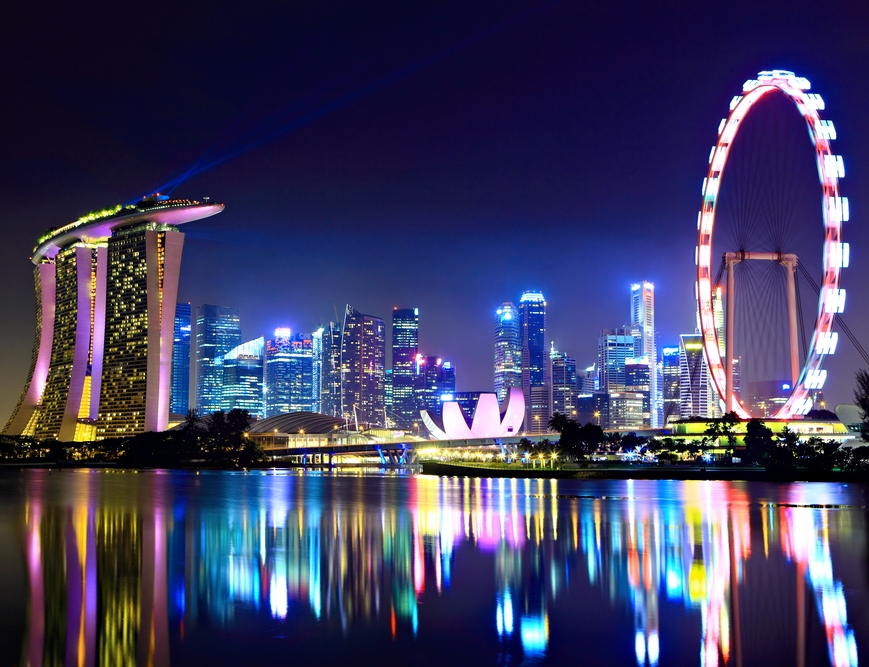
\includegraphics[width=\textwidth]{singapore.jpg}

    
    \section*{Introduction}\label{Introduction}

   

    On the particular project, I am using data mungling techniques to assess
the quality of OpenStreetMap's (OSM) data for the center of Singapore
regarding their consistency and uniformity. The data wrangling takes
place programmatically, using \textbf{Python} for the most of the
process and \textbf{SQL} for items that need further attention while in
the \textbf{PostgreSQL}.\\

    

    The dataset describes the center of Singapore, covering an area from
Clementi on the west, to Bedok on the east and from Serangoon on the
north, to Sentosa Island on the south. The size of the dataset is 96 MB
and can can be downloaded from
\href{http://overpass-api.de/api/map?bbox=103.7651,1.2369,103.9310,1.3539}{here}\\

\begin{center}\color{brown}\rule{1\linewidth}{\linethickness}\end{center}


    \section*{Data Assessment}\label{data-assessment}

     An initial exploration of the dataset revealed the following problems:
\begin{itemize}
 \item Abbreviations of street types like `Av' instead of `Avenue' and `Rd'
instead of `Road'.
\end{itemize}
\begin{itemize}
 \item All lowercase letters like `street' instead of `Street'.
\end{itemize}
\begin{itemize}
 \item Postcodes including the first letter (S xxxxxx) or the whole name (Singapore xxxxxx) of the country.
\end{itemize}
\begin{itemize}
 \item Postcodes omitting the leading `0' (probably because of declared as integers at some point before their import to OpenStreetMap.)
\end{itemize}
\begin{itemize}
 \item Multi-abbreviated amenity names.
\end{itemize}
The problems in the amenity names were to a small extent, and they were
corrected directly in the database, the rest resolved programmatically
using Python on the biggest part and a subtle portion of them needed
further assessment, resolven in the database.


    \subsection*{Auditing Street Types}\label{auditing-street-types}

    To audit the Street Types I need to extract the Street Names from the
XML.

The Street Names appear in two forms in the dataset:

In \emph{Node} and \emph{Way} elements, in the form of: ``\emph{\textless{} tag k=``addr:street''
v=``\textbf{street\_name}''/\textgreater{}}''

    \begin{Shaded}
\begin{Highlighting}[]
\OperatorTok{<}\NormalTok{node }\BuiltInTok{id}\OperatorTok{=}\StringTok{"337171253"} \NormalTok{lat}\OperatorTok{=}\StringTok{"1.3028023"} \NormalTok{lon}\OperatorTok{=}\StringTok{"103.8599300"} \NormalTok{version}\OperatorTok{=}\StringTok{"3"} 
\NormalTok{timestamp}\OperatorTok{=}\StringTok{"2015-08-01T01:38:25Z"} \NormalTok{changeset}\OperatorTok{=}\StringTok{"33022579"} \NormalTok{uid}\OperatorTok{=}\StringTok{"741163"}
\NormalTok{user}\OperatorTok{=}\StringTok{"JaLooNz"}\OperatorTok{>}
    \OperatorTok{<}\NormalTok{tag k}\OperatorTok{=}\StringTok{"addr:city"} \NormalTok{v}\OperatorTok{=}\StringTok{"Singapore"}\OperatorTok{/>}
    \OperatorTok{<}\NormalTok{tag k}\OperatorTok{=}\StringTok{"addr:country"} \NormalTok{v}\OperatorTok{=}\StringTok{"SG"}\OperatorTok{/>}
    \OperatorTok{<}\NormalTok{tag k}\OperatorTok{=}\StringTok{"addr:housenumber"} \NormalTok{v}\OperatorTok{=}\StringTok{"85"}\OperatorTok{/>}
    \OperatorTok{<}\NormalTok{tag k}\OperatorTok{=}\StringTok{"addr:postcode"} \NormalTok{v}\OperatorTok{=}\StringTok{"198501"}\OperatorTok{/>}
    \OperatorTok{<}\NormalTok{tag k}\OperatorTok{=}\StringTok{"addr:street"} \NormalTok{v}\OperatorTok{=}\StringTok{"Sultan Gate"}\OperatorTok{/>}
  \OperatorTok{</}\NormalTok{node}\OperatorTok{>}
\end{Highlighting}
\end{Shaded}

    In \emph{Way} elements that have the ``\emph{\textless{} tag k=''highway"
\ldots{}./\textgreater{}}``, and the `\emph{v}' attribute is one of
{[}`living\_street', `motorway', `primary', `residential', `secondary',
`tertiary'{]}, as''\emph{\textless{} tag k=``name''
v=``\textbf{street\_name}''/\textgreater{}}``.

    \begin{Shaded}
\begin{Highlighting}[]
\OperatorTok{<}\NormalTok{way }\BuiltInTok{id}\OperatorTok{=}\StringTok{"4386520"} \NormalTok{version}\OperatorTok{=}\StringTok{"23"} \NormalTok{timestamp}\OperatorTok{=}\StringTok{"2016-11-07T12:03:39Z"}
\NormalTok{changeset}\OperatorTok{=}\StringTok{"43462870"} \NormalTok{uid}\OperatorTok{=}\StringTok{"2818856"} \NormalTok{user}\OperatorTok{=}\StringTok{"CitymapperHQ"}\OperatorTok{>}
    \OperatorTok{<}\NormalTok{nd ref}\OperatorTok{=}\StringTok{"4486796339"}\OperatorTok{/>}
    \OperatorTok{<}\NormalTok{nd ref}\OperatorTok{=}\StringTok{"1278204303"}\OperatorTok{/>}
    \OperatorTok{<}\NormalTok{nd ref}\OperatorTok{=}\StringTok{"3689717007"}\OperatorTok{/>}
    \OperatorTok{<}\NormalTok{nd ref}\OperatorTok{=}\StringTok{"246494174"}\OperatorTok{/>}
    \OperatorTok{<}\NormalTok{tag k}\OperatorTok{=}\StringTok{"highway"} \NormalTok{v}\OperatorTok{=}\StringTok{"primary"}\OperatorTok{/>}
    \OperatorTok{<}\NormalTok{tag k}\OperatorTok{=}\StringTok{"name"} \NormalTok{v}\OperatorTok{=}\StringTok{"Orchard Road"}\OperatorTok{/>}
    \OperatorTok{<}\NormalTok{tag k}\OperatorTok{=}\StringTok{"oneway"} \NormalTok{v}\OperatorTok{=}\StringTok{"yes"}\OperatorTok{/>}
  \OperatorTok{</}\NormalTok{way}\OperatorTok{>}
\end{Highlighting}
\end{Shaded}

    Although most of the Singaporean street names end with the street type
(e.g., ``Serangoon Road'' or ``Arab Street'') it is also common to end
with a number instead (e.g. ``Bedok North Avenue 1''). Thus, by using
regular expressions, I am extracting from the streetnames, the last word that does not contain
numbers.

    It would be easy to populate the list of Common Street Types with some
profound values like Street or Avenue, but guessing does not take into
account any local peculiarity. Instead, I searched the dataset for all
the different types and used the 12 with the most occurrences (From 13th
position, abbreviations start to appear).



    \begin{longtable}[c]{@{}lllllllll@{}}
\toprule
& Street Type & Occurrences & & Street Type & Occurrences & & Street
Type & Occurrences\tabularnewline
\midrule
\endhead
1 & `Road' & 574 & 6 & `Geylang' & 42 & 11 & `Link' & 34\tabularnewline
2 & `Avenue' & 145 & 7 & `Crescent' & 42 & 12 & `Terrace' &
30\tabularnewline
3 & `Street' & 139 & 8 & `Walk' & 40 & 13 & `Ave' & 29\tabularnewline
4 & `Drive' & 87 & 9 & `Park' & 39 & 14 & `Hill' & 25\tabularnewline
5 & `Lane' & 80 & 10 & `Close' & 37 & 15 & `Flyover' & 23\tabularnewline
\bottomrule
\end{longtable}

    To find the street names that need correction, I used the
``get\_close\_matches()'' function from the
\href{https://docs.python.org/2/library/difflib.html?highlight=get_close_matches}{``difflib''}
module to find ``close matches'' of the 12 Common Street Types. This is
what I found:

    \begin{Shaded}
\begin{Highlighting}[]
\NormalTok{Road [}\StringTok{'Road'}\NormalTok{, }\StringTok{'road'}\NormalTok{, }\StringTok{'Rd'}\NormalTok{, }\StringTok{'Ria'}\NormalTok{]  }
\NormalTok{Avenue [}\StringTok{'Avenue'}\NormalTok{, }\StringTok{'Aenue'}\NormalTok{, }\StringTok{'Avebue'}\NormalTok{, }\StringTok{'Ave'}\NormalTok{]  }
\NormalTok{Street [}\StringTok{'Street'}\NormalTok{, }\StringTok{'street'}\NormalTok{, }\StringTok{'See'}\NormalTok{, }\StringTok{'Stangee'}\NormalTok{]  }
\NormalTok{Drive [}\StringTok{'Drive'}\NormalTok{, }\StringTok{'Grove'}\NormalTok{, }\StringTok{'Grisek'}\NormalTok{, }\StringTok{'Bridge'}\NormalTok{]  }
\NormalTok{Lane [}\StringTok{'Lane'}\NormalTok{, }\StringTok{'Lana'}\NormalTok{, }\StringTok{'Lateh'}\NormalTok{, }\StringTok{'Layang'}\NormalTok{]  }
\NormalTok{Geylang [}\StringTok{'Geylang'}\NormalTok{, }\StringTok{'Pelangi'}\NormalTok{, }\StringTok{'Selangat'}\NormalTok{, }\StringTok{'Selanting'}\NormalTok{]  }
\NormalTok{Crescent [}\StringTok{'Crescent'}\NormalTok{, }\StringTok{'Cresent'}\NormalTok{, }\StringTok{'Cres'}\NormalTok{, }\StringTok{'Green'}\NormalTok{]  }
\NormalTok{Walk [}\StringTok{'Walk'}\NormalTok{, }\StringTok{'walk'}\NormalTok{, }\StringTok{'Wajek'}\NormalTok{, }\StringTok{'Wakaff'}\NormalTok{]  }
\NormalTok{Park [}\StringTok{'Park'}\NormalTok{, }\StringTok{'park'}\NormalTok{, }\StringTok{'Parkway'}\NormalTok{, }\StringTok{'Paras'}\NormalTok{]  }
\NormalTok{Close [}\StringTok{'Close'}\NormalTok{, }\StringTok{'Cross'}\NormalTok{, }\StringTok{'Circle'}\NormalTok{, }\StringTok{'Flyover'}\NormalTok{]  }
\NormalTok{Link [}\StringTok{'Link'}\NormalTok{, }\StringTok{'link'}\NormalTok{, }\StringTok{'Minyak'}\NormalTok{, }\StringTok{'Bingka'}\NormalTok{]  }
\NormalTok{Terrace [}\StringTok{'Terrace'}\NormalTok{, }\StringTok{'Terrance'}\NormalTok{, }\StringTok{'Ter'}\NormalTok{, }\StringTok{'service'}\NormalTok{]}
\end{Highlighting}
\end{Shaded}

    The Python code was able to correct 998 problems both in addresses where
the Street Type was at the end of the address\\
\texttt{Greenwood\ Ave\ ==\textgreater{}\ Greenwood\ Avenue\ (2\ occurrences)}\\
and wher it was not:\\
\texttt{Eunos\ Ave\ 7A\ ==\textgreater{}\ Eunos\ Avenue\ 7A}

    \subsection*{Auditing Postcodes}\label{auditing-postcodes}

    Postcodes in Singapore consist of 6 digits with the first two, denoting
the Postal Sector and taking values between 01 and 80, excluding 74
(\href{https://www.ura.gov.sg/realEstateIIWeb/resources/misc/list_of_postal_districts.htm}{link}).\\
I searched the dataset for this pattern, correcting whatever could be
addressed automatically and added the rest to the ``PROBLEMATICS'' for
further examination.\\
Postcodes were much more consistent than the street types with 3
problems fixed programmatically and 8 pending further inspection.

    \begin{center}\color{brown}\rule{1\linewidth}{\linethickness}\end{center}

    \section*{Assessment in the Database}\label{assessment-in-the-database}

    After performing the most of the cleaning with Python, I stored the
dataset in a database to explore it and examine further the PROBLEMATIC
elements.

    As a database I used PostgreSQL to present a generic solution although a
lightweight database like SQLite might be a more appropriate choice for
the size of the dataset.

    \subsection*{Addresses}\label{addresses}

    The small number of the elements that were requiring further attention
(13) allowed me to examine them one by one. There were three categories of
problems.\\
In the first category belong elements that some values have been placed
to wrong attributes (e.g.~housenumber in the place of postcode. These
problems resolved just by checking the attributes and update the
relevant tables with the righ keys/values relation.\\
Incomplete addresses with no self-explained errors belong to the second
category. For these elements I defined a function that uses Google Maps
API to resolve the full address from a partial address. This was helpful
for the addresses with missing postcodes.\\
Finally, whatever could not be resolved with one of the above ways I
used web search with any information available.

    You may find the changes that took place during this phase in the
following table.

\newpage

\begin{longtable}[c]{@{}llll@{}}
\toprule
Element id & Problematic Attribute & Original Value & Corrected
Value\tabularnewline
\midrule
\endhead
453243296 & street & 2 & (street attribute removed)\tabularnewline
453243296 & housenumber & (missing) & 2\tabularnewline
453253763 & street & 2 & (street attribute removed)\tabularnewline
453253763 & housenumber & (missing) & 2\tabularnewline
453227146 & street & 65 & Alexandra Terrace\tabularnewline
46649997 & street & 65 & Alexandra Terrace\tabularnewline
169844052 & street & 310074 & Lor 4 Toa Payoh\tabularnewline
169844052 & postcode & 74 & 310074\tabularnewline
169844052 & housenumber & (missing) & 74\tabularnewline
1318498347 & postcode & 135 & (postcode attribute
removed)\tabularnewline
1318498347 & housenumber & (missing) & 135\tabularnewline
3026819436 & postcode & 2424 & 238841\tabularnewline
3756813987 & postcode & 05901 & 059011\tabularnewline
4338649392 & postcode & 88752 & 088752\tabularnewline
4338649392 & housenumber & (missing) & 279\tabularnewline
4338649392 & street & (missing) & New Bridge Road\tabularnewline
4496749591 & postcode & \#B1-42 & (element deleted)\tabularnewline
23946435 & postcode & 437 437 & 437437\tabularnewline
172769494 & postcode & 05901 & 059011\tabularnewline
\bottomrule
\end{longtable}

    \subsection*{Amenities}\label{amenities}

    In Singapore they refer to the banks with their abbreviations rather
than their complete names. This fact along with their popularity of the
ATMs on the street amenities list (will be presented later) makes them
prone to mistakes. The assessment revealed only 5 issues:
\begin{itemize}
 \item `UOB' referred as `Uob'
\end{itemize}
\begin{itemize}
 \item `POSB' referred as `Posb'
\end{itemize}
\begin{itemize}
 \item `OCBC' referred as `Overseas Chinese Banking Corporation'
\end{itemize}
\begin{itemize}
 \item 2 completely irrelevant nodes marked as `ATM'
\end{itemize}

    \begin{center}\color{brown}\rule{1\linewidth}{\linethickness}\end{center}

    \section*{Data Exploration}\label{data-exploration}

    \subsection*{Dataset Specific}\label{dataset-specific}

    \textbf{Size of the database}

    \begin{Verbatim}[commandchars=\\\{\}]
{\color{incolor}In [{\color{incolor}15}]:} \PY{n}{size\PYZus{}in\PYZus{}bytes} \PY{o}{=} \PY{o}{\PYZpc{}}\PY{k}{sql} SELECT pg\PYZus{}database\PYZus{}size(\PYZsq{}Project\PYZus{}3\PYZsq{});
         \PY{k}{print} \PY{l+s+s2}{\PYZdq{}}\PY{l+s+s2}{DB size: }\PY{l+s+s2}{\PYZdq{}} \PY{o}{+} \PY{n+nb}{str}\PY{p}{(}\PY{n}{size\PYZus{}in\PYZus{}bytes}\PY{p}{[}\PY{l+m+mi}{0}\PY{p}{]}\PY{p}{[}\PY{l+m+mi}{0}\PY{p}{]}\PY{o}{/}\PY{l+m+mi}{1024}\PY{o}{*}\PY{o}{*}\PY{l+m+mi}{2}\PY{p}{)} \PY{o}{+} \PY{l+s+s1}{\PYZsq{}}\PY{l+s+s1}{ MB}\PY{l+s+s1}{\PYZsq{}}
\end{Verbatim}

    \begin{Verbatim}[commandchars=\\\{\}]
DB size: 96 MB

    \end{Verbatim}

    \textbf{Number of Unique Users}

    \begin{Verbatim}[commandchars=\\\{\}]
{\color{incolor}In [{\color{incolor}24}]:} \PY{o}{\PYZpc{}\PYZpc{}}\PY{k}{sql}
         SELECT count(DISTINCT(uid)) AS \PYZdq{}Unique Users\PYZdq{}
         FROM (SELECT uid FROM nodes
               UNION SELECT uid FROM ways) AS elements
\end{Verbatim}

            \begin{Verbatim}[commandchars=\\\{\}]
{\color{outcolor}Out[{\color{outcolor}24}]:} [(847L,)]
\end{Verbatim}
        
    \textbf{Number of \emph{Nodes} and \emph{Ways}}

    \begin{Verbatim}[commandchars=\\\{\}]
{\color{incolor}In [{\color{incolor}18}]:} \PY{n}{n\PYZus{}nodes} \PY{o}{=} \PY{o}{\PYZpc{}}\PY{k}{sql} SELECT COUNT(*) FROM nodes
         \PY{n}{n\PYZus{}ways} \PY{o}{=} \PY{o}{\PYZpc{}}\PY{k}{sql} SELECT COUNT(*) FROM ways
         
         \PY{k}{print} \PY{l+s+s2}{\PYZdq{}}\PY{l+s+s2}{Number of }\PY{l+s+s2}{\PYZsq{}}\PY{l+s+s2}{nodes: }\PY{l+s+s2}{\PYZdq{}} \PY{o}{+} \PY{n+nb}{str}\PY{p}{(}\PY{n}{n\PYZus{}nodes}\PY{p}{[}\PY{l+m+mi}{0}\PY{p}{]}\PY{p}{[}\PY{l+m+mi}{0}\PY{p}{]}\PY{p}{)}
         \PY{k}{print} \PY{l+s+s2}{\PYZdq{}}\PY{l+s+s2}{Number of }\PY{l+s+s2}{\PYZsq{}}\PY{l+s+s2}{ways: }\PY{l+s+s2}{\PYZdq{}} \PY{o}{+} \PY{n+nb}{str}\PY{p}{(}\PY{n}{n\PYZus{}ways}\PY{p}{[}\PY{l+m+mi}{0}\PY{p}{]}\PY{p}{[}\PY{l+m+mi}{0}\PY{p}{]}\PY{p}{)}
\end{Verbatim}

    \begin{Verbatim}[commandchars=\\\{\}]
Number of 'nodes: 409350
Number of 'ways: 66404

    \end{Verbatim}

    \subsection*{Area Specific}\label{area-specific}

    \textbf{Most frequent amenities}

    No surprises here, Singaporeans love food! Restaurant are the first
amenity with nearly 3 times more occurrences from the second amenity.

    \begin{Verbatim}[commandchars=\\\{\}]
{\color{incolor}In [{\color{incolor}23}]:} \PY{o}{\PYZpc{}\PYZpc{}}\PY{k}{sql}
         SELECT value AS \PYZdq{}Amenity\PYZdq{}, COUNT(value) AS \PYZdq{}Occurrences\PYZdq{}
         FROM (SELECT * FROM nodes\PYZus{}tags
               UNION ALL SELECT * FROM nodes\PYZus{}tags) AS tags
         WHERE key = \PYZsq{}amenity\PYZsq{}
         GROUP BY value
         ORDER BY \PYZdq{}Occurrences\PYZdq{} DESC
         LIMIT 10
\end{Verbatim}

            \begin{Verbatim}[commandchars=\\\{\}]
{\color{outcolor}Out[{\color{outcolor}23}]:}
	  [(u'restaurant', 1562L),
          (u'parking', 654L),
          (u'taxi', 524L),
          (u'cafe', 396L),
          (u'fast\_food', 252L),
          (u'atm', 190L),
          (u'toilets', 190L),
          (u'bar', 176L),
          (u'bank', 120L),
          (u'police', 120L)]
\end{Verbatim}


        
    \paragraph{Most popular cuisine}\label{most-popular-cuisine}

    \begin{Verbatim}[commandchars=\\\{\}]
{\color{incolor}In [{\color{incolor}8}]:} \PY{o}{\PYZpc{}\PYZpc{}}\PY{k}{sql}
        SELECT value AS \PYZdq{}Cuisine\PYZdq{}, COUNT(*) AS \PYZdq{}Restaurants\PYZdq{} 
        FROM (SELECT * FROM nodes\PYZus{}tags 
              UNION ALL 
              SELECT * FROM ways\PYZus{}tags) tags
        WHERE tags.key=\PYZsq{}cuisine\PYZsq{}
        GROUP BY value
        ORDER BY \PYZdq{}Restaurants\PYZdq{}  DESC
        LIMIT 10
\end{Verbatim}

            \begin{Verbatim}[commandchars=\\\{\}]
{\color{outcolor}Out[{\color{outcolor}8}]:} [(u'chinese', 99L),
         (u'japanese', 42L),
         (u'korean', 36L),
         (u'coffee\_shop', 34L),
         (u'burger', 33L),
         (u'italian', 32L),
         (u'indian', 28L),
         (u'asian', 27L),
         (u'pizza', 17L),
         (u'french', 15L)]
\end{Verbatim}
        
    \paragraph{Religion}\label{religion}

    Singapore is well-known for its multicultural environment. People with
different religious and ethnic heritages are forming the modern
city-state. This is reflected in the variety of temples that can be
found in the country.

    \begin{Verbatim}[commandchars=\\\{\}]
{\color{incolor}In [{\color{incolor}25}]:} \PY{o}{\PYZpc{}\PYZpc{}}\PY{k}{sql}
         SELECT tags.value AS \PYZdq{}Religion\PYZdq{}, COUNT(*) AS \PYZdq{}Temples\PYZdq{} 
         FROM (SELECT * FROM nodes\PYZus{}tags
               UNION ALL 
               SELECT * FROM ways\PYZus{}tags) tags
         WHERE tags.key=\PYZsq{}religion\PYZsq{}
         GROUP BY tags.value
         ORDER BY \PYZdq{}Temples\PYZdq{} DESC;
\end{Verbatim}

            \begin{Verbatim}[commandchars=\\\{\}]
{\color{outcolor}Out[{\color{outcolor}25}]:} [(u'christian', 73L),
          (u'muslim', 38L),
          (u'buddhist', 30L),
          (u'hindu', 9L),
          (u'taoist', 6L),
          (u'jewish', 1L),
          (u'sikh', 1L)]
\end{Verbatim}
        
    \begin{center}\color{brown}\rule{1\linewidth}{\linethickness}\end{center}

    \section*{Ideas for additional
improvements.}\label{ideas-for-additional-improvements.}

    There are two areas where the current project can be improved in the
future. The first one is on the completeness of the data. All the above
analysis is based on a dataset that reflects a big part of Singapore but
not the whole country. The reason for this is the lack of a way to
download a dataset big enough to include the entire Singapore without
including parts of the neighboring countries.\\
As a future improvement, I would download the metro extract from
\href{https://mapzen.com/data/metro-extracts/metro/singapore/}{MapZen}
and filter the non-Singaporean nodes and their references. The filtering
would involve the creation of polygons from a suitable shapefile like
\href{http://www.diva-gis.org/gdata}{this one} with a GIS library like
\href{https://pypi.python.org/pypi/Fiona}{Fiona} and the comparison of
\emph{Nodes}' coordinates with these polygons with a geometric library
like \href{https://github.com/Toblerity/Shapely}{Shapely}.\\
The drawback of the above technique is that the comparison of each node
against the polygons is a very time-consuming procedure with my initial
tests taking 17-18 hours to produce a result.

    The second area with room for future improvement is the exploratory
analysis. Although the scope of the current project was the wrangling of
the dataset, thus the exploration has been kept in a basic level, the
dataset is full of information that can be extracted. Just to mention
some:\\
- Distribution of commits per contributor. - Plotting of element
creation date, per type, per day. - Popular franchises in the country
(fast food, conventional stores, etc.)

And even more interesting such us:

\begin{itemize}
\tightlist
\item
  Distribution of distance between different types of amenities.
\item
  Selection of a bank based on the average distance you have to walk for
  an ATM.
\item
  Which area has the biggest parks and recreation spaces.
\end{itemize}

    \subsection*{References}\label{references}

    Udacity - https://www.udacity.com/\\
Wikipedia - https://www.wikipedia.org/\\
OpenStreetMap - https://www.openstreetmap.org\\
Overpass API - http://overpass-api.de/\\
Python Software Foundation - https://www.python.org/\\
Urban Redevelopment Authority of Singapore - https://www.ura.gov.sg\\
Catherine Devlin's Github repository -
https://github.com/catherinedevlin/ipython-sql


    % Add a bibliography block to the postdoc
    
    
    
    \end{document}
